\documentclass[10pt,a4paper,twocolumn]{article}
\usepackage[utf8]{inputenc}
\usepackage{amsmath}
\usepackage{amsfonts}
\usepackage{amssymb}
\usepackage{graphicx}
\usepackage{hyperref}
\usepackage{listings}
\usepackage{float}
\usepackage[dutch]{babel}
\author{Ruben Van Assche}
\graphicspath{ {../plots/} }
\title{Data Smoothing - Oefening 5}
\date{\today}
\begin{document}
\maketitle
\section{Software}
Doorheen deze opgave heb ik gebruik gemaakt van GSL\footnote{\url{https://www.gnu.org/software/gsl/}}. Alle functies in deze opgave gebruikt komen dan ook uit de \texttt{\detokenize{gsl_rng}} , \texttt{\detokenize{gsl_linalg}}, \texttt{\detokenize{gsl_sf_legendre}} workspace.
\section{Opgave}
Het doel van deze opgave bestond er in om het polynomiale kleinste kwadraten model van graad 2 te berekenen. De x punten worden gegeven in het interval $[-1,1]$ en worden voorgesteld door volgende functie : $x_{i} = -1 + \frac{i}{100}$ met $i = 0,\hdots,200$. De y punten door volgende functie : $y(x) = 1 + 2x + x^{2}$. Dit levert volgende plot op :
\begin{figure}[H]
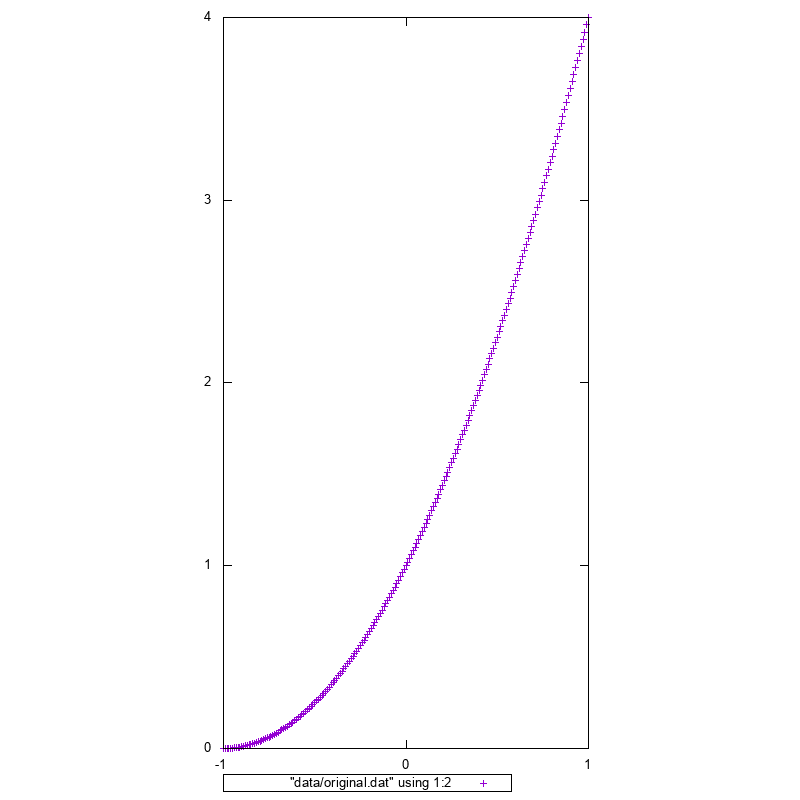
\includegraphics[width=0.4\textwidth]{original}
\end{figure}
Een deel van de opgave was om ruis toe te voegen aan de datapunten. Deze ruis moest liggen in het interval $[-1, 1]$ en uniform verdeeld zijn. De functie die GSL hiervoor voorziet is \texttt{\detokenize{gsl_rng_uniform}}, deze levert een waarde $r$ op in interval $[0,1)$. Het eerste wat gebeurt is het herschalen van $r$ naar het interval $[-1, 1]$ d.m.v. volgende vergelijking : $r*2-1$. Als random number generator koos ik voor \texttt{\detokenize{gsl_rng_mt19937}}. Wanneer we de ruis optellen bij de gegenereerde punten bekomen we volgende plot:
\begin{figure}[H]
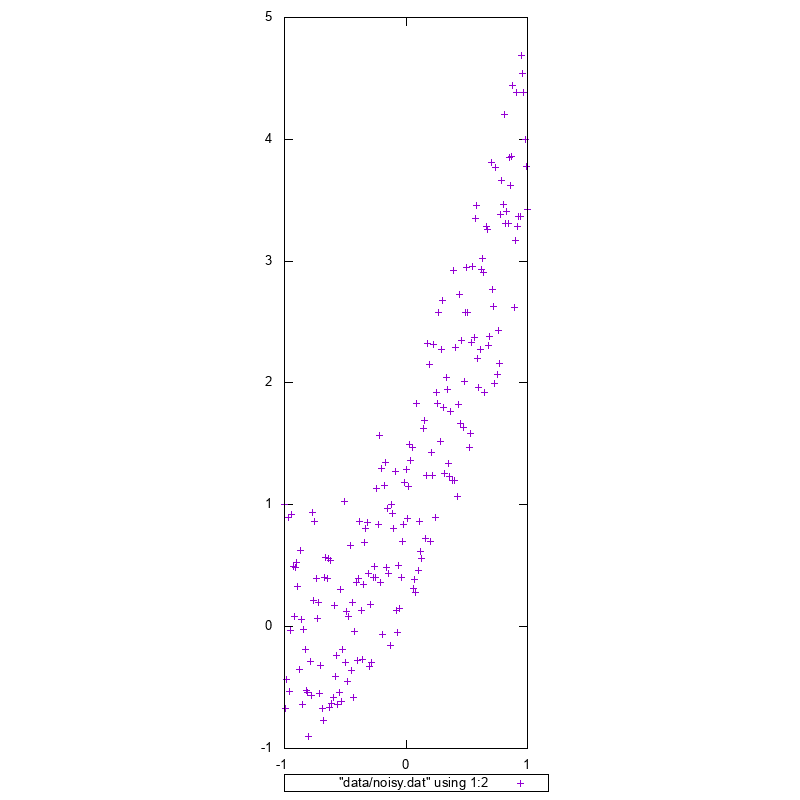
\includegraphics[width=0.4\textwidth]{noisy}
\end{figure}
Letterlijk een "wolk" van datapunten.
\section{Opstellen kleinste kwadraten model}
Zoals in de cursus wordt aangegeven zullen we bij het kleinste kwadraten model de $l_{2}$ norm van het residu($r = y - A\lambda$) proberen te minimaliseren. Wanneer dit wordt uitgevoerd bij matrices bekomen we volgende formule:
$$(A^{T}A)\gamma = A^{T}y$$
Dit lineair systeem is zeer slecht geconditioneerd, dus het oplossen ervan zal geen betrouwbare oplossing geven. Een oplossing bestaat erin om gebruik te maken van QR factorisatie, hierbij zal een decompositie van A in Q en R plaatsvinden. Waardoor d.m.v. volgende functie de minimale $l_{2}$ norm van het residu berekend kan worden:
$$min \left \| Ax -y \right \|_{2} = min\left \|Q^{T}Ax -Q^{T}y  \right \|_{2} $$
$$= \sqrt{\sum_{i=n+1}^{m}(Q^{T}y)_{i}^{2}}$$
GSL voorziet voor de decompositie de \texttt{\detokenize{gsl_linalg_QR_decomp}} functie en voor het oplossen van het stelsel waarbij de $l_{2}$ norm van het residu wordt geminimaliseerd de \texttt{\detokenize{gsl_linalg_QR_lssolve}} functie. Het polynomiale kleinste kwadraten model ziet er dan alsvolgt uit :
$$1 + \lambda_{1} *x +\lambda_{2}* x^{2}$$
Een kleine opmerking die gemaakt moet worden: in de cursus wordt gebruik gemaakt van Givens rotations voor de QR factorisatie. De functie \texttt{\detokenize{gsl_linalg_QR_decomp}} in GSL maakt gebruik van Householder rotations. Ik heb alle libraries(Numerical Recipes, GAMS, Netlib) doorzocht naar een functie waarbij de QR factorisatie wordt uitgevoerd met een Givens rotation maar kon deze helaas niet vinden.
\subsection{Originele punten}
Als eerste bekijken we de originele punten(zonder ruis). Hiervoor gebruiken we volgend model:
$$
A \lambda = \begin{bmatrix}
1 & x_{0} & x^{2}_{0} \\ 
\vdots &  & \vdots\\ 
1 & x_{200} & x^{2}_{200}
\end{bmatrix}
* \begin{bmatrix}
\lambda_{0} \\
\lambda_{1}  \\
\lambda_{2} 
\end{bmatrix}
= \begin{bmatrix}
y_{0} \\
\vdots  \\
y_{200}
\end{bmatrix}
$$
Dit levert dan volgende vergelijking op:
$$1 + 2x + 1x^2$$
Wat natuurlijk exact hetzelfde is zoals gegeven, de $l_{2}$ norm van het residu is 7.26249e-15 wat natuurlijk te verwachten is gezien de functie hetzelfde is als de gegeven functie.  Hetzelfde geldt voor de $l_{2}$ norm van de error welke 4.43742e-15 is. Een plot:
\begin{figure}[H]
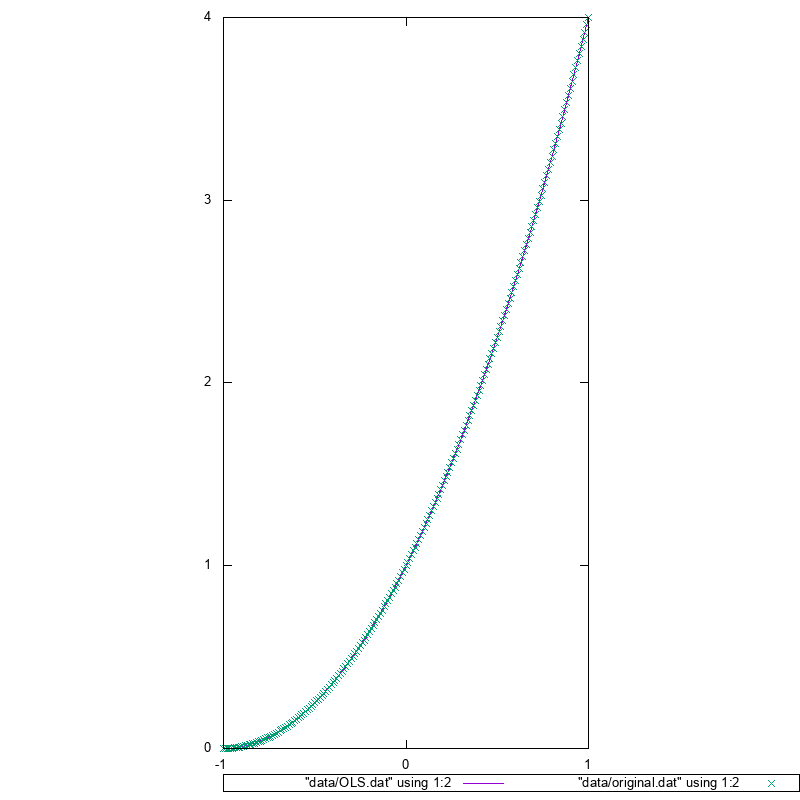
\includegraphics[width=0.4\textwidth]{OLS}
\end{figure}
\subsection{Noisy Punten}
Laat ons opnieuw het model toepassen met als verschil dat deze keer gebruik wordt gemaakt van de punten $y$ met ruis:
$$
A \lambda = \begin{bmatrix}
1 & x_{0} & x^{2}_{0} \\ 
\vdots &  & \vdots\\ 
1 & x_{200} & x^{2}_{200}
\end{bmatrix}
* \begin{bmatrix}
\lambda_{0} \\
\lambda_{1}  \\
\lambda_{2} 
\end{bmatrix}
= \begin{bmatrix}
y_{0} \\
\vdots  \\
y_{200}
\end{bmatrix}
$$
Dit levert een verschillende vergelijking op:
$$0.885437 + 2.07339x + 1.1688x^{2}$$
Wanneer we nu naar de $l_{2}$ norm van het residu kijken bekomen we 7.79653. Hierbij hebben we als $y$ waarde in $r = y - A\lambda$ gebruik gemaakt van de punten zonder ruis, dit omdat we deze punten willen benaderen met het model. En niet de punten met ruis. De residu vector volledig staat achteraan. Zoals verwacht is natuurlijk de $l_{2}$ norm van de error groter geworden en is deze hier 1.24651. Wanneer dit wordt geplot zien we dat de functie mooi doorheen de wolk van punten gaat en dus probeert de $l_{2}$ norm van het residu te minimaliseren.
\begin{figure}[H]
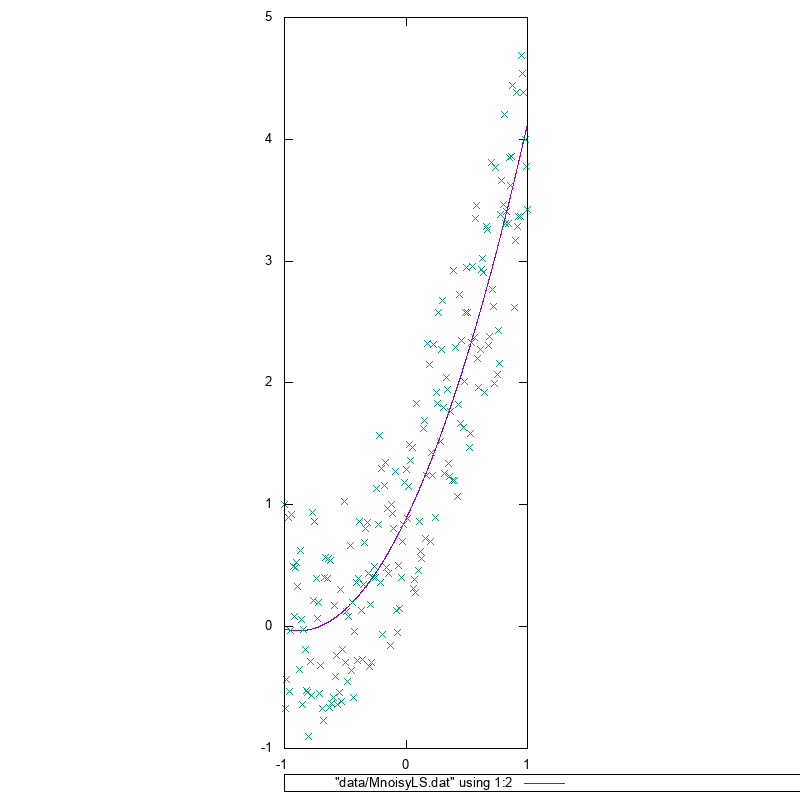
\includegraphics[width=0.4\textwidth]{MnoisyLS}
\end{figure}
Als laatste is het misschien interessant om zowel de originele als de met ruis least squares approximation te plotten op één afbeelding:
\begin{figure}[H]
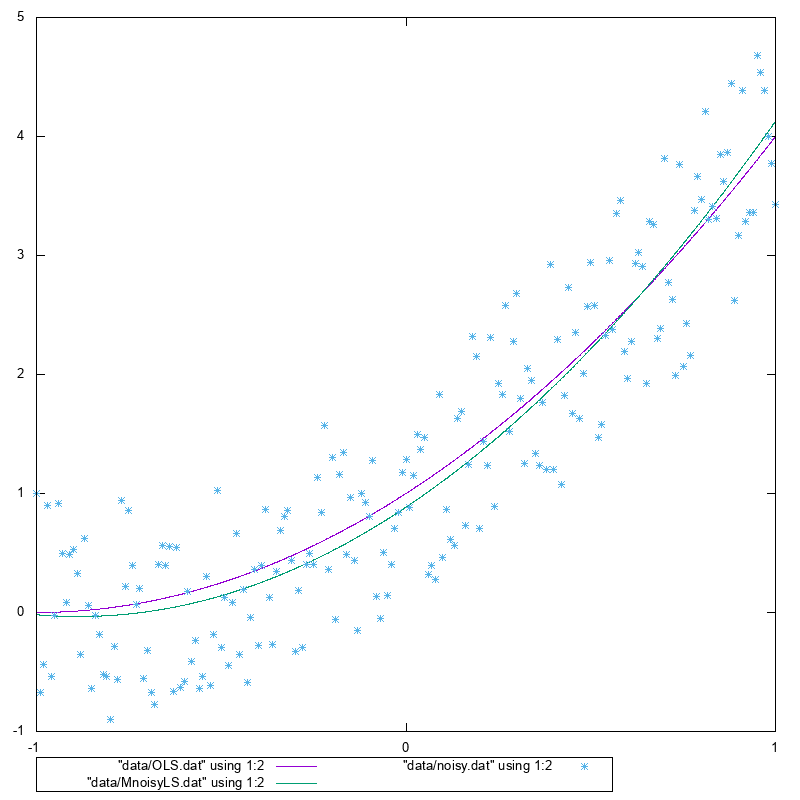
\includegraphics[width=0.4\textwidth]{monomialsCombinedLS}
\end{figure}
\section{Residu's}
\subsection{Originele Punten}
0, -1.11022e-16, -1.11022e-16, -1.11022e-16, -1.11022e-16, -1.11022e-16, -1.11022e-16, 0, 0, 0, 0, 0, 0, 0, 0, 0, 0, 0, 0, 0, 0, 1.11022e-16, 1.11022e-16, 1.11022e-16, 1.11022e-16, 1.11022e-16, 1.11022e-16, 1.11022e-16, 1.11022e-16, 1.11022e-16, 1.11022e-16, 1.11022e-16, 1.11022e-16, 1.11022e-16, 1.66533e-16, 1.66533e-16, 1.66533e-16, 1.66533e-16, 1.66533e-16, 1.66533e-16, 1.66533e-16, 1.66533e-16, 1.66533e-16, 1.66533e-16, 1.66533e-16, 2.22045e-16, 2.22045e-16, 2.22045e-16, 2.22045e-16, 2.22045e-16, 2.22045e-16, 2.22045e-16, 2.22045e-16, 2.22045e-16, 2.77556e-16, 2.77556e-16, 2.77556e-16, 2.77556e-16, 2.22045e-16, 2.22045e-16, 2.22045e-16, 2.77556e-16, 2.22045e-16, 3.33067e-16, 2.77556e-16, 2.77556e-16, 2.77556e-16, 3.33067e-16, 2.77556e-16, 2.77556e-16, 2.77556e-16, 3.33067e-16, 3.33067e-16, 2.22045e-16, 3.33067e-16, 3.33067e-16, 3.33067e-16, 2.22045e-16, 3.33067e-16, 3.33067e-16, 3.33067e-16, 3.33067e-16, 3.33067e-16, 3.33067e-16, 3.33067e-16, 3.33067e-16, 2.22045e-16, 3.33067e-16, 3.33067e-16, 3.33067e-16, 3.33067e-16, 3.33067e-16, 3.33067e-16, 3.33067e-16, 3.33067e-16, 3.33067e-16, 3.33067e-16, 3.33067e-16, 3.33067e-16, 3.33067e-16, 3.33067e-16, 4.44089e-16, 4.44089e-16, 4.44089e-16, 4.44089e-16, 4.44089e-16, 4.44089e-16, 4.44089e-16, 4.44089e-16, 4.44089e-16, 4.44089e-16, 4.44089e-16, 4.44089e-16, 4.44089e-16, 4.44089e-16, 4.44089e-16, 4.44089e-16, 4.44089e-16, 4.44089e-16, 4.44089e-16, 4.44089e-16, 4.44089e-16, 4.44089e-16, 4.44089e-16, 4.44089e-16, 4.44089e-16, 4.44089e-16, 4.44089e-16, 4.44089e-16, 4.44089e-16, 4.44089e-16, 4.44089e-16, 4.44089e-16, 4.44089e-16, 4.44089e-16, 4.44089e-16, 4.44089e-16, 2.22045e-16, 2.22045e-16, 4.44089e-16, 4.44089e-16, 4.44089e-16, 4.44089e-16, 4.44089e-16, 4.44089e-16, 4.44089e-16, 0, 0, 4.44089e-16, 4.44089e-16, 4.44089e-16, 4.44089e-16, 4.44089e-16, 4.44089e-16, 0, 4.44089e-16, 4.44089e-16, 0, 4.44089e-16, 4.44089e-16, 4.44089e-16, 4.44089e-16, 4.44089e-16, 4.44089e-16, 0, 4.44089e-16, 4.44089e-16, 4.44089e-16, 4.44089e-16, 0, 0, 4.44089e-16, 4.44089e-16, 0, 4.44089e-16, 0, 0, 4.44089e-16, 0, 4.44089e-16, 0, 4.44089e-16, 0, 4.44089e-16, 0, 0, 4.44089e-16, 4.44089e-16, 0, 4.44089e-16, 0, 0, 4.44089e-16, 0, 0, 0, 0, 0, 0, 0, 0
\subsection{Noisy Punten}
0.0191613, 0.0217864, 0.0243778, 0.0269354, 0.0294592, 0.0319493, 0.0344056, 0.0368281, 0.0392169, 0.041572, 0.0438933, 0.0461808, 0.0484345, 0.0506545, 0.0528408, 0.0549933, 0.057112, 0.0591969, 0.0612481, 0.0632656, 0.0652493, 0.0671992, 0.0691154, 0.0709978, 0.0728464, 0.0746613, 0.0764424, 0.0781898, 0.0799034, 0.0815833, 0.0832293, 0.0848417, 0.0864202, 0.0879651, 0.0894761, 0.0909534, 0.0923969, 0.0938067, 0.0951827, 0.096525, 0.0978335, 0.0991082, 0.100349, 0.101556, 0.10273, 0.10387, 0.104975, 0.106048, 0.107086, 0.108091, 0.109062, 0.109999, 0.110902, 0.111772, 0.112608, 0.11341, 0.114178, 0.114913, 0.115614, 0.116281, 0.116914, 0.117513, 0.118079, 0.118611, 0.11911, 0.119574, 0.120005, 0.120402, 0.120765, 0.121094, 0.12139, 0.121652, 0.12188, 0.122075, 0.122235, 0.122362, 0.122456, 0.122515, 0.122541, 0.122532, 0.122491, 0.122415, 0.122306, 0.122162, 0.121985, 0.121775, 0.12153, 0.121252, 0.12094, 0.120594, 0.120215, 0.119802, 0.119355, 0.118874, 0.118359, 0.117811, 0.117229, 0.116613, 0.115964, 0.115281, 0.114563, 0.113813, 0.113028, 0.11221, 0.111358, 0.110472, 0.109552, 0.108599, 0.107612, 0.106591, 0.105536, 0.104448, 0.103325, 0.102169, 0.10098, 0.0997563, 0.0984991, 0.0972081, 0.0958834, 0.0945249, 0.0931326, 0.0917066, 0.0902468, 0.0887533, 0.087226, 0.0856649, 0.0840701, 0.0824415, 0.0807792, 0.0790831, 0.0773533, 0.0755897, 0.0737923, 0.0719612, 0.0700963, 0.0681976, 0.0662652, 0.064299, 0.0622991, 0.0602654, 0.058198, 0.0560968, 0.0539618, 0.0517931, 0.0495906, 0.0473544, 0.0450844, 0.0427806, 0.0404431, 0.0380718, 0.0356667, 0.0332279, 0.0307554, 0.0282491, 0.025709, 0.0231352, 0.0205276, 0.0178862, 0.0152111, 0.0125022, 0.00975958, 0.00698318, 0.00417303, 0.00132912, -0.00154855, -0.00445999, -0.00740518, -0.0103841, -0.0133968, -0.0164433, -0.0195235, -0.0226375, -0.0257853, -0.0289668, -0.032182, -0.0354311, -0.0387139, -0.0420304, -0.0453807, -0.0487648, -0.0521826, -0.0556342, -0.0591195, -0.0626386, -0.0661915, -0.0697781, -0.0733985, -0.0770526, -0.0807405, -0.0844622, -0.0882176, -0.0920068, -0.0958297, -0.0996864, -0.103577, -0.107501, -0.111459, -0.115451, -0.119476, -0.123536, -0.127629
\end{document}